\documentclass[rgb,dvipsnames]{beamer}
\usepackage[english]{babel}
\usepackage{xcolor}
\usepackage{listings}
\usepackage{adjustbox}

\usepackage{amsmath}

\usepackage[linewidth=1pt]{mdframed}

% Graphics
\usepackage{graphicx}

% Font
\usepackage{paratype}
\setbeamerfont{frametitle}{family=\bf}
\usefonttheme[onlymath]{serif}

\newcommand{\nn}{\mathcal{N}}
\newcommand{\uu}{\mathcal{U}}
\newcommand{\bb}{\mathcal{B}}
\newcommand{\ee}{\mathrm{e}}
\newcommand{\rd}[1]{\mathrm{#1}}
\newcommand{\bd}[1]{\mathbf{#1}}  % for bolding symbols
\newcommand{\RR}{\mathbb{R}}      % for Real numbers
\newcommand{\ZZ}{\mathbb{Z}}      % for Integers
\newcommand{\BB}{\mathbb{B}}      % for Booleans
\newcommand{\PP}{\mathbb{P}}      % for Prob
\newcommand{\EE}{\mathbb{E}}      % for Expectation
\newcommand{\II}{\mathbbm{1}}      % for Indicator fun
\newcommand{\NN}{\mathbb{N}}      % for Prob
\newcommand{\col}[1]{\left[\begin{matrix} #1 \end{matrix} \right]}
\newcommand{\comb}[2]{\binom{#1^2 + #2^2}{#1+#2}}

\usepackage{tikz}
\usetikzlibrary{arrows,fit, positioning, shapes,
  calc, fadings, decorations.pathmorphing, hobby}

\tikzset{font=\tiny}
\tikzset{terminal/.style={circle, draw=black, fill=black, text=white}}
\tikzset{steiner/.style={circle, draw=black, fill=white}}
\tikzset{selected/.style={draw=red, ultra thick}}
\tikzset{assignment/.style={draw=red, thin, opacity=0.6}}
\tikzset{root/.style={draw=cyan, ultra thick}}
\tikzset{subgraph/.style={font=\large, text=gray}}
\tikzset{snake it/.style={-stealth,
    decoration={snake, 
      amplitude = .2mm,
    segment length = 2mm,
    post length=0.9mm},decorate}}
\tikzset{snake node/.style={above=1mm,
    midway,
    text width=3cm,
    sloped,
    align=center}}


% Beamer theme settings
\usetheme{Copenhagen}
\usecolortheme{seagull}
\setbeamertemplate{itemize item}{\raisebox{0.8mm}{\rule{1.2mm}{1.2mm}}}
\usenavigationsymbolstemplate{} % no navigation buttons

\mode<presentation>
{ \usetheme{boxes} }

\title{Master's Thesis Defense}
\subtitle{The Prize-Collecting Steiner Tree Problem
  \\and Related Problems}
\author{William Jack Lysgaard Sprent}
\date{31st August 2018}
\institute{DIKU}
\begin{document}

\AtBeginSection[]
{
   \begin{frame}
       \frametitle{Outline}
       \tableofcontents[currentsection]
   \end{frame}
 }
 
\frame{\titlepage}

\begin{frame}{The fun we are having today:}
\tableofcontents
\end{frame}

\section{Introduction}

\begin{frame}{Overview}{What happened in the last six months?}
  \pause
  \begin{itemize}
  \item I read a stack of research papers about the PCSTP. \pause
  \item I read a smaller stack of research papers about related problems. \pause
  \item \textit{I was indecisive.} \pause
  \item I worked on a solver for the Median Tree Problem.
  \end{itemize}
\end{frame}

\begin{frame}{Motivation}{Why the PCSTP?}
  \begin{itemize}
  \item It's a hard problem. Hard problems are worth solving.
  \item It relates to the Steiner Tree Problem, and shares some of
    its characteristica.
    \pause
  \item Finally: \textit{It is an interesting problem.}
  \end{itemize}
\end{frame}

\begin{frame}{Motivation}{The Survey}
  What makes a survey necessary?
  \pause
  \begin{itemize}
  \item A lot is written about the PCSTP, but it is unstructured and disjoint.
  \item Some of these papers touch on very complex subjects
    and are sometimes short and unintuitive.
  \item The PCSTP is a good ``case study'' for an ILP problem.
  \end{itemize}
  \pause
  \textbf{ --- There is a lot to learn.}
  
\end{frame}

\begin{frame}{Motivation}{Why the Median Tree Problem?}
  \pause
  \textit{We'll get back to that later.}
\end{frame}
\section{The Prize-Collecting Steiner Tree Problem}
\begin{frame}{The Prize-Collecting Steiner Tree Problem}{Short History}
  \begin{itemize}
  \item Defined by Egon Balas in 1988 as a side effect.
  \item Subject to steady focus in the late 90's and early 00's.
  \item One of the subjects of the 11th DIMACs Implementation Challenge in 2014.
  \end{itemize}
\end{frame}
\begin{frame}{The Prize-Collecting Steiner Tree Problem}{Problem Definition}
 Given an undirected graph
\[G = (V, E, c, p)\]
where $c: E \to \RR^+$ defines edge weights,
and $p: V \to \RR^+$ defines vertex \textit{prizes}, then the solution to the
\textit{PCSTP} is a tree
\[T = (V_T, E_T, c, p) \subseteq G\]
which minimizes
\[c(T) = \min_T \sum_{(i,j) \in E_T} c_{ij} + \sum_{v\in (V \setminus V_T)} p_v \textnormal{.} \]
\end{frame}

\begin{frame}{The Prize-Collecting Steiner Tree Problem}{Example}
  \centering
  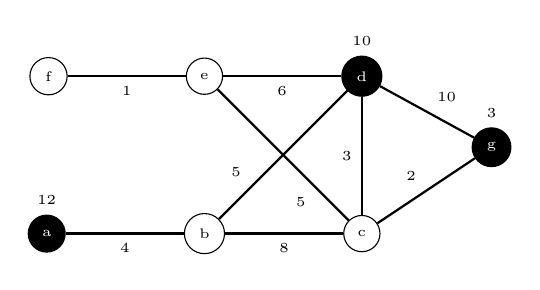
\begin{tikzpicture}[auto, node distance=1.5 cm]
  %Nodes
  \node[terminal, label={12}] (a) {a};
  \node[steiner] (b) [right=of a] {b};
  \node[steiner] (c) [right=of b] {c};
  \node[terminal, label={10}] (d) [above =of c] {d};
  \node[steiner] (e) [left=of d] {e};
  \node[steiner] (f) [left=of e] {f};
  \node[terminal, label={3}] (g) [above right=0.75 and 1.3 of c] {g};
  % Edges
  \begin{scope}[every edge/.style={draw=black, thick}]
    \draw (a) edge node[below]{4} (b);
    \draw (b) edge node[near start]{5} (d);
    \draw (b) edge node[below]{8} (c);
    \draw (c) edge node{3} (d);
    \draw (c) edge node{2} (g);
    \draw (c) edge node[near start]{5} (e);
    \draw (d) edge node{6} (e);
    \draw (d) edge node{10} (g);
    \draw (e) edge node{1} (f);
  \end{scope}
\end{tikzpicture}
\end{frame}

\begin{frame}{The Prize-Collecting Steiner Tree Problem}{Example}
  \centering
  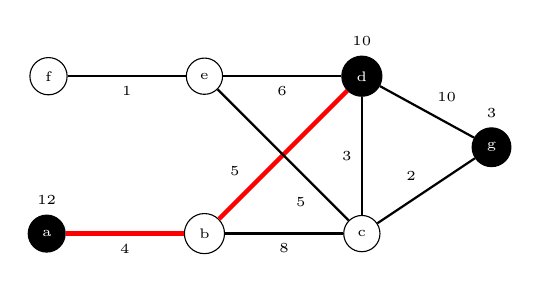
\begin{tikzpicture}[auto, node distance=1.5 cm]
  %Nodes
  \node[terminal, label={12}] (a) {a};
  \node[steiner] (b) [right=of a] {b};
  \node[steiner] (c) [right=of b] {c};
  \node[terminal, label={10}] (d) [above =of c] {d};
  \node[steiner] (e) [left=of d] {e};
  \node[steiner] (f) [left=of e] {f};
  \node[terminal, label={3}] (g) [above right=0.75 and 1.3 of c] {g};
  % Edges
  \begin{scope}[every edge/.style={draw=black, thick}]
    \draw (a) edge[selected] node[below]{4} (b);
    \draw (b) edge[selected] node[near start]{5} (d);
    \draw (b) edge node[below]{8} (c);
    \draw (c) edge node{3} (d);
    \draw (c) edge node{2} (g);
    \draw (c) edge node[near start]{5} (e);
    \draw (d) edge node{6} (e);
    \draw (d) edge node{10} (g);
    \draw (e) edge node{1} (f);
  \end{scope}
\end{tikzpicture}

\end{frame}
\begin{frame}{The Survey}{Quick Summary}

  \begin{block}{Contents of the Survey:}
  \begin{enumerate}
  \item The history of solving the PCSTP.
  \item Preprocessing routines.
  \item Two heuristic algorithms. LP-based and search based.
  \item An approximation algorithm: the GW Algorithm.
  \item How to separate GSECs.
  \item The DHEA and SCIP-Jack solvers.
  \end{enumerate}
\end{block}
\end{frame}

\begin{frame}{The Survey}{Main Points}
  \begin{block}{What have we learned?}
    \pause
    \begin{enumerate}
    \item The PCSTP is well covered all things considered. \pause
  \item Preprocessing is \textit{very} good for the PCSTP. \pause
  \item Directed formulations of the problem are preferable for
    branch and bound. \pause
  \item Heuristics are aplenty.
  \end{enumerate}
  \end{block}

\end{frame}

\begin{frame}{The Survey}{Main Points}
  \begin{block}{Curiosities}
  \begin{itemize}
  \item Not a lot of focus on applications.
  \item Linear progress?
  \item Somewhat general methods besides preprocessing.
  \end{itemize}
\end{block}
\pause
\textit{On to other problems.}
\end{frame}

\section{Other Ways of Collecting Prize}
\begin{frame}{Prize-Collecting Tours}
  \begin{block}{Three main variants:}
    \begin{enumerate}
    \item The Prize-Collecting Travelling Salesman Problem
    \item The Orienteering Problem
    \item The Profitable Tour Problem
    \end{enumerate}
  \end{block}
  \pause
  \begin{block}{Some Notes:}
  \begin{itemize}
  \item Main point of the Balas paper in 88.
  \item Shares approximation algorithms.
  \item Apart from the OP, not well covered.
  \end{itemize}
\end{block}

\end{frame}

\begin{frame}{Median Subgraphs}
  \begin{itemize}
  \item Assignment Problem.
  \item Different shapes of facility.
  \item Median Trees.
  \end{itemize}
\end{frame}

\begin{frame}{Summary}
  \begin{itemize}
  \item Two axis' of similarity: structure and prize function.
  \item PCSTP is the most well researched problem in the family.
  \end{itemize}
  \pause
  \textbf{What now?}
\end{frame}

\section{The Median Tree Problem}
\begin{frame}{Motivation}{Options}
  \begin{itemize}
  \item Stay with the PCSTP.
  \item Look at the Profitable Tour Problem.
  \item Look at the Median Tree Problem.
  \end{itemize}
\end{frame}
\begin{frame}{Motivation}{Median Trees over Prize-Collecting Tours}
  \begin{itemize}
  \item A feasible solution to the PCSTP is a feasible solution to the MTP.
  \item Collect Prize vs. Assignment: similar --- although not the exact same --- trade offs.
  \end{itemize}
  \pause
 \textit{And a splash of subjectivity.}
\end{frame}
\begin{frame}{Median Tree Problem}{Problem Definition}
  Let $G = (V, E, c, d)$ be an undirected graph. Denote $c : E \to \RR^+$ as an \textit{edge cost} function
and $d : V \times V  \to \RR^+$ be an \textit{assignment cost} function where we have
\[d_{ii} = 0 \mathnormal{.}\]
Then the \textit{Median Tree Problem}
is defined as finding a \textit{connected subgraph} $T = (V_T, E_T)$ of $G$
where $V_T \subseteq V$ and
$E_T \subseteq E$ which minimises the cost function,
\[c(T) = \sum_{ij \in E_T} c_{ij} + \sum_{i \in V} \min_{j \in V_T} d_{ij}\mathnormal{.}\]
\end{frame}

\begin{frame}{Median Tree Problem}{ILP Formulation}
  \begin{subequations}
    \small
     \begin{alignat}{3}
       &\underset{\bd x, \bd y}{\text{minimize}}
       & & \sum_{ij \in E} c_{ij} x_{ij} +  \sum_{i, j \in V} d_{ij}y_{ij}  & \\
       & \text{subject to}\quad
       & & \sum_{ij \in E} x_{ij} = \sum_{i \in V} y_{ii} - 1 &&  \label{form:mtp:tree}\\
       &&& x(E(S)) \leq \sum_{i \in S \setminus \{s\}} y_{ii}
       && \forall S \subseteq V, s \in S \label{form:mtp:gsec} \\
       &&& \sum_{j \in V} y_{kj} = 1 && \forall k \in V \label{form:mtp:assignment}\\
       &&& y_{ik} \leq  y_{kk}
       && \forall i, k \in V \label{form:mtp:facility}\\
       &&& y_{kk} \leq \sum_{i \in \delta(k)} x_{ik}
       && \forall k \in V \label{form:mtp:legal} \\
       &&& \bd x \in \BB^{|E|} && \\
       &&& \bd y \in \BB^{|V \times V|}
     \end{alignat}
   \end{subequations}
 \end{frame}
    \normalsize
 \begin{frame}{Median Tree Problem}{Valid Inequalities}
\pause
\textit{Forced self-assignment:}
\[
 y_{ii} \geq x_{ji} \qquad \forall i \in V,  \forall j \in \delta(i)\mathnormal{.}
\]
\pause
\textit{Degree of Nonterminals:}
\[
   \sum_{j \in \delta(i)}x_{ij} \geq 2 x_{ik} \qquad \forall i \in N, \: \forall k \in \delta(i)
\]


 \end{frame}
\begin{frame}{The Solver}
  \begin{itemize}
  \item Based on the Gurobi MIP solver. \pause
  \item Callbacks written in Python 3. \pause
  \item Applies methods from the PCSTP survey: \pause
    \begin{itemize}
    \item Primal heuristic from the DHEA solver.
    \item User cuts based on GSEC separation from an
      article by Lucena and Resende for the PCSTP.
    \end{itemize}
  \end{itemize}
  
\end{frame}
\begin{frame}{Results}
  
\end{frame}
\section{Summary / Reflections}
\begin{frame}{What did I manage to do?}
  haha
\end{frame}

\begin{frame}{Improvements}{The Survey}
  
\end{frame}

\begin{frame}{Improvements}{The Solver}
  
\end{frame}

\begin{frame}{Further Work}{Solve a real problem}
  haha
\end{frame}


\begin{frame}{Lessons Learned}
  
\end{frame}

\begin{frame}{Postface}
  \large\textbf{Questions?}
\end{frame}
\end{document}